\documentclass[convert=pdf2svg]{standalone}
\usepackage{tikz}

\usetikzlibrary{intersections,arrows.meta}

\renewcommand{\familydefault}{\sfdefault}

\begin{document}

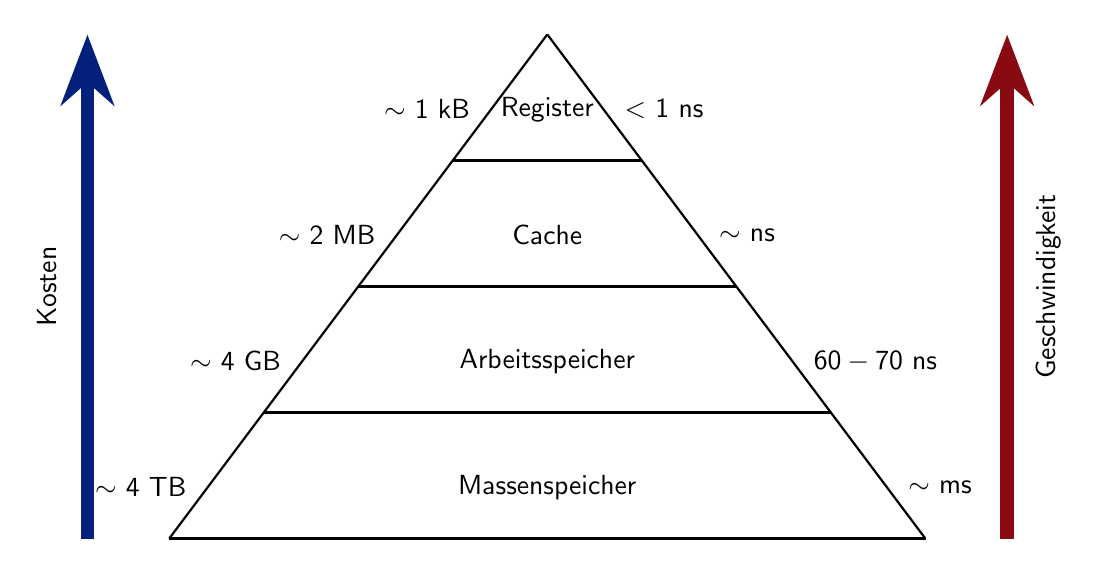
\begin{tikzpicture}[scale=1.6]
\definecolor{my_blue}{RGB}{80,116,172}
\definecolor{my_blue_dark}{RGB}{3,33,122}
\definecolor{my_blue_light}{RGB}{163,203,240}

\definecolor{my_orange}{RGB}{217,132,92}
\definecolor{my_orange_dark}{RGB}{173,64,35}
\definecolor{my_orange_light}{RGB}{251,180,139}

\definecolor{my_green}{RGB}{91,166,108}
\definecolor{my_green_dark}{RGB}{32,112,42}
\definecolor{my_green_light}{RGB}{148,228,167}

\definecolor{my_red}{RGB}{192,80,86}
\definecolor{my_red_dark}{RGB}{136,11,17}	
\definecolor{my_red_light}{RGB}{251,159,158}	

\definecolor{my_violet}{RGB}{128,116,174}
\definecolor{my_violet_dark}{RGB}{87,34,108}	
\definecolor{my_violet_light}{RGB}{207,189,250}

\definecolor{my_brown}{RGB}{145,120,100}
\definecolor{my_brown_dark}{RGB}{159,187,159}	
\definecolor{my_brown_light}{RGB}{87,47,21}

\definecolor{my_pink}{RGB}{215,141,192}
\definecolor{my_pink_dark}{RGB}{247,177,225}	
\definecolor{my_pink_light}{RGB}{158,56,127}

\definecolor{my_gray}{RGB}{140,140,140}
\definecolor{my_gray_dark}{RGB}{60,60,60}
\definecolor{my_gray_light}{RGB}{207,207,207}

\definecolor{my_yellow}{RGB}{203,184,125}
\definecolor{my_yellow_dark}{RGB}{255,253,175}	
\definecolor{my_yellow_light}{RGB}{182,132,48}

\definecolor{my_turkis}{RGB}{106,181,202}
\definecolor{my_turkis_dark}{RGB}{189,242,240}	
\definecolor{my_turkis_light}{RGB}{20,99,114}

\coordinate (A) at (-3,0) {};
\coordinate (B) at ( 3,0) {};
\coordinate (C) at (0,4) {};
\draw[name path=AC, thick] (A) -- (C);
\draw[name path=BC, thick] (B) -- (C);

\def\velsr{{"$\sim$ ms","$\sf 60-70$ ns","$\sim$ ns","$<$ 1 ns"}};
\def\velsl{{"$\sim$ 4 TB", "$\sim$ 4 GB", "$\sim$ 2 MB", "$\sim$ 1 kB"}};
%\def\vels{{"$\sim$ ms","$\sim$ ms","$\sim$ ms","$\sim$ ms"}};

\foreach \y/\A [count=\xi from 0] in {0/Massenspeicher,1/Arbeitsspeicher,2/Cache,3/Register} {
    \pgfmathsetmacro\vellabr{\velsr[\xi]}
    \pgfmathsetmacro\vellabl{\velsl[\xi]}
    \path[name path=horiz] (A|-0,\y) -- (B|-0,\y);
    \draw[name intersections={of=AC and horiz,by=P},
          name intersections={of=BC and horiz,by=Q}, thick] (P) node[left=-0.35cm, above=0.65cm,anchor=east] {\vellabl} -- (Q)
        node[midway,above=0.65cm, anchor=center] {\A} node[right=-0.35cm, above=0.65cm,anchor=west] {\vellabr};

}
\draw[->,-Stealth, thick,my_blue_dark,line width=5pt] (-3.65,0)--+(0,4);
\node[left=0.2cm, rotate=90, anchor=center] at (-3.85,2) {Kosten};
\draw[->,-Stealth, thick, my_red_dark,line width=5pt] (3.65,0)--+(0,4);
\node[right=0.2cm, rotate=90, anchor=center] at (3.85,2) {Geschwindigkeit};
\end{tikzpicture}
\end{document}